\chapter{Methods}
\label{ch:methods}

In the method of this thesis, a clip of film music is mapped to eight predicted emotion ratings, and the film's genres are predicted from these eight values alone (audio $\rightarrow$ 8 emotions $\rightarrow$ genre). The main experiments compare this two-stage route with the same audio representation given directly to the same genre classifier, and with a control that compresses the representation to eight dimensions without any reference to emotion. Two datasets are used. The film-music dataset of \citet{eerola2011comparison} provides the audio and the emotion ratings, and the Blockbuster dataset of \citet{ma2021computational} provides an independent set of films for testing. This chapter describes the data and their genre labels (Section~\ref{sec:methods_data}), the audio representations (Section~\ref{sec:methods_features}), the two models of the pipeline (Sections~\ref{sec:methods_stage1} and~\ref{sec:methods_stage2}), the baselines and controls (Section~\ref{sec:methods_baselines}), the evaluation protocol (Section~\ref{sec:evaluation_protocol}) and the implementation (Section~\ref{sec:methods_implementation}). Figure~\ref{fig:pipeline} gives an overview. The underlying concepts are explained in Chapter~\ref{ch:fundamentals}; this chapter describes what was done.

\begin{figure}[t]
  \centering
  \resizebox{\textwidth}{!}{%
  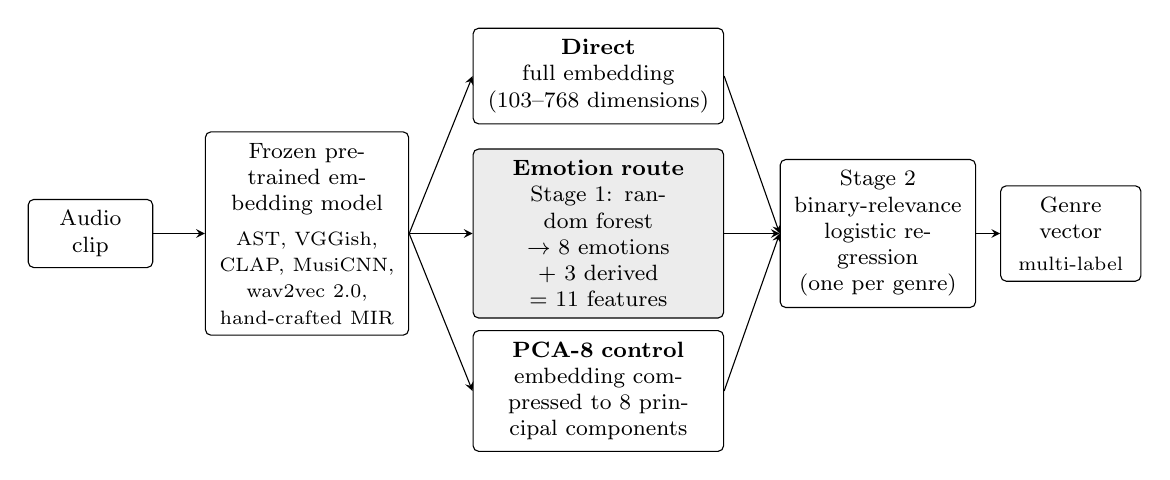
\begin{tikzpicture}[font=\footnotesize, >=stealth,
      box/.style={draw, rounded corners=2pt, align=center, inner sep=4pt}]
    % input and frozen front-end
    \node[box, text width=1.3cm] (audio) at (0,0) {Audio\\clip};
    \node[box, text width=2.3cm] (emb) at (2.75,0)
      {Frozen pretrained embedding model\\[3pt]\scriptsize AST, VGGish, CLAP, MusiCNN, wav2vec~2.0, hand-crafted MIR};
    % the three routes
    \node[box, text width=2.9cm] (direct) at (6.45,2.0)
      {\textbf{Direct}\\full embedding\\(103--768 dimensions)};
    \node[box, text width=2.9cm, fill=gray!15] (emo) at (6.45,0)
      {\textbf{Emotion route}\\Stage~1: random forest\\$\rightarrow$ 8 emotions + 3 derived\\$=$ 11 features};
    \node[box, text width=2.9cm] (pca) at (6.45,-2.0)
      {\textbf{PCA-8 control}\\embedding compressed to 8 principal components};
    % one shared classifier and the output
    \node[box, text width=2.2cm] (clf) at (10.0,0)
      {Stage~2\\binary-relevance logistic regression\\(one per genre)};
    \node[box, text width=1.5cm] (genre) at (12.45,0)
      {Genre\\vector\\[2pt]\scriptsize multi-label};
    % arrows
    \draw[->] (audio) -- (emb);
    \draw[->] (emb.east) -- (direct.west);
    \draw[->] (emb.east) -- (emo.west);
    \draw[->] (emb.east) -- (pca.west);
    \draw[->] (direct.east) -- (clf.west);
    \draw[->] (emo.east) -- (clf.west);
    \draw[->] (pca.east) -- (clf.west);
    \draw[->] (clf) -- (genre);
  \end{tikzpicture}}
  \caption{The two-stage pipeline, the direct baseline and the PCA-8 control.}
  \label{fig:pipeline}
\end{figure}

All three routes in Figure~\ref{fig:pipeline} start from the same frozen embedding and end in the same Stage~2 classifier, trained and tuned identically; only the input of that classifier differs. The emotion route (shaded) is the method under test and the direct route is the baseline. The PCA-8 route is a control that is as narrow as the emotion route but has no emotional meaning.

\section{Datasets}
\label{sec:methods_data}

\subsection{The Eerola Film Soundtrack Dataset}
\label{subsec:methods_eerola}

The primary dataset is the film-music set published by \citet{eerola2011comparison}. Its first set (Set~1) contains 360 clips of film music from 45 soundtracks, between 10 and 31\,s long (mean 17\,s). Each clip was rated by a listener panel on eight emotion scales, each from 1 to 9: the three dimensional scales valence, energy and tension, and the five discrete emotions anger, fear, happiness, sadness and tenderness (Section~\ref{sec:fund_models}). The target of the first pipeline stage is the panel mean for each scale. As explained in Section~\ref{sec:fund_emotion_def}, these are ratings of \emph{perceived} emotion, i.e.\ what the listeners judged the music to express rather than what they felt.

The second set (Set~2) contains 110 clips from Set~1, rated again by a different listener panel. Of these, 102 clips from 38 soundtracks can be matched clip by clip. On them, the panels agree with a mean correlation of $r=0.912$ and a consistency intraclass correlation, ICC(C,1), of 0.897, which is taken as the ceiling on the $R^2$ an audio model can be expected to reach (Section~\ref{sec:eval_emotion}). Set~2 serves only to estimate how reliable the ratings are and plays no part in training or evaluation.

The dataset has no genre information. Genre labels were added from the Internet Movie Database (IMDb), using the identifier of the film each soundtrack belongs to. The annotation is the film's genre list, so all clips of a film carry the same labels: a gentle cue from an Action film is labelled Action. This is one reason why every split in this thesis is grouped by film (Section~\ref{sec:evaluation_protocol}).

\subsection{The Blockbuster Dataset}
\label{subsec:methods_blockbuster}

The second dataset, by \citet{ma2021computational}, contains 110 commercially successful films released between 2014 and 2019, each labelled with one or more of six genres (Action, Drama, Comedy, Sci-Fi, Romance and Horror). The dataset is used in two ways. In-domain, the published result is reproduced with the classifier of this thesis, which validates the classifier against an external benchmark. Across datasets, it is an independent test set of unseen films, on which the claim that emotion generalises is tested.

For copyright reasons, the Blockbuster dataset contains no audio. Instead, the authors publish features pre-extracted from each musical \emph{cue} (one continuous piece of score music as it is used in the film): a 128-dimensional VGGish embedding and 140 hand-crafted MIR descriptors per cue. The dataset contains 4664 cues, with a median of 39 per film and a median length of 19\,s. As a result, none of the other representations of Section~\ref{sec:methods_features} can be computed for these films. VGGish is the only representation available on both datasets, so it is used in every experiment that crosses them. A cue is also the same kind of object as an Eerola clip, a stretch of score music of comparable length. The emotion regressor, which is trained on Eerola clips, is therefore applied to each cue individually, and the predicted emotions are averaged per film afterwards. If the embeddings were first averaged over the film and emotion predicted only once, the regressor would receive a much smoother vector than anything it saw in training.

\subsection{Genre Labels}
\label{subsec:genre_labels}

Genre is treated as a multi-label problem throughout (Section~\ref{sec:fund_ml}). IMDb lists a film's genres roughly in alphabetical order rather than by relevance, so the first-listed genre is not a ``primary'' genre. No such notion is used, and a clip carries every modelled genre its film is listed with. Clips enter a label space under an \emph{any-present} rule. A clip is kept if at least one of its IMDb genres belongs to the modelled set, and it is then labelled with all genres that do. Clips whose film has no modelled genre (for example, only Fantasy or Mystery) are excluded from that label space. They still have emotion ratings and are included when Stage~1 is evaluated on its own.

This gives three label spaces, which are summarised in Table~\ref{tab:label_spaces}. Since they differ in their genres, clips and chance levels, a score from one space cannot be compared with a score from another. Every result in Chapter~\ref{ch:evaluation} is therefore given with its label space and the chance floor of that space.

In Table~\ref{tab:label_spaces}, the entries are the number of clips carrying each genre (Eerola) or the number of films (Blockbuster), and a dash means that the genre is not part of that space.

\paragraph{(a) The eight-genre Eerola space.} Eight genres occur often enough in the Eerola films to be modelled: Action, Adventure, Biography, Comedy, Crime, Documentary, Drama and Horror. Together they give 346 clips from 42 films. The labels are strongly imbalanced: Drama applies to 239 clips, Documentary to 17.

\paragraph{(b) The five-genre subset.} In prior work on film audio, the number of modelled genres grows with the size of the dataset. At a scale comparable to this one, \citet{austin2010characterization} model four genres over 98 films, and \citet{ma2021computational}, who also work from soundtracks, reduce the IMDb genres to six for their 110 films. The eighteen-genre study of \citet{mangolin2020multimodal} and the nine-genre study of \citet{behrouzi2023multimodal} rest on thousands of films. Compared with this, eight genres from 42 soundtracks is ambitious, and three of them are poorly supported. Biography and Documentary have fewer than 25 clips each. Adventure is frequent but has no distinctive emotional signature (every $|d| \le 0.25$; Section~\ref{sec:eval_signatures}), so it is unlikely to be recoverable from emotional features. Results are therefore reported both on all eight genres and on a curated subset of five (Action, Crime, Drama, Comedy and Horror), which are established in the literature and have a measurable emotional signature here. Under the any-present rule the subset contains 329 clips from 40 films. The eight-genre results show the limits imposed by rare and affectively indistinct genres; the five-genre results describe performance where the approach is applicable and form the main in-domain setting.

\paragraph{(c) The six-genre space shared with Blockbuster.}
A model can only be transferred between two datasets if it predicts the same classes in both. The two genre inventories differ, however: Crime, Adventure, Biography and Documentary do not exist in the Blockbuster annotation, and Sci-Fi and Romance are not among the eight Eerola genres. Both datasets are therefore relabelled into one shared space of six genres, namely Action, Drama, Comedy, Sci-Fi, Romance and Horror. These six were adopted from \citet{ma2021computational} rather than chosen here, and the rule they used to reduce the IMDb genres to them was recovered from their published film--genre master list rather than assumed. It is the identity rule: a film carries reduced genre $g$ if and only if $g$ occurs in its raw IMDb genre list, which holds for all 110 of their films without exception. This is the any-present rule already applied to the Eerola annotations, so both datasets enter the shared space under the same rule and without any dataset-specific heuristic. On Eerola it retains 319 clips from 41 films.

\begin{table}[t]
  \centering
  \small
  \caption{The three genre label spaces.}
  \label{tab:label_spaces}
  \begin{tabular}{lrrrr}
    \toprule
     & (a) Eerola & (b) Eerola & \multicolumn{2}{c}{(c) shared space} \\
    Genre & 8 genres & 5 genres & Eerola & Blockbuster \\
    \midrule
    Action      & 103 & 103 & 103 & 55 \\
    Adventure   &  97 & --  & --  & -- \\
    Biography   &  24 & --  & --  & -- \\
    Comedy      &  40 &  40 &  40 & 37 \\
    Crime       &  98 &  98 & --  & -- \\
    Documentary &  17 & --  & --  & -- \\
    Drama       & 239 & 239 & 239 & 44 \\
    Horror      &  28 &  28 &  28 & 11 \\
    Romance     & --  & --  &  51 & 13 \\
    Sci-Fi      & --  & --  &  19 & 36 \\
    \midrule
    Clips (films) & 346 (42) & 329 (40) & 319 (40) & 110 films \\
    Used for    & in-domain & in-domain (main) & \multicolumn{2}{c}{transfer} \\
    \bottomrule
  \end{tabular}
\end{table}

\section{Audio Representations}
\label{sec:methods_features}

Six audio representations are compared, so that a conclusion about ``direct audio'' does not rest on one possibly poorly chosen model. Five are frozen pretrained networks and one is a hand-crafted baseline without any pretraining. The networks cover four pretraining regimes: general sound events (AST, VGGish), audio--text matching (CLAP), music tagging (MusiCNN) and speech (wav2vec~2.0). Section~\ref{sec:fund_audio} describes each model, and Table~\ref{tab:representations} lists what was used.

\begin{table}[t]
  \centering
  \small
  \caption{The six audio representations.}
  \label{tab:representations}
  \setlength{\tabcolsep}{4pt}
  \begin{tabular}{lllll}
    \toprule
    Representation & Input & Pretraining data & Audio used & Dim. \\
    \midrule
    AST         & log-mel spectrogram & AudioSet            & first 10.24\,s & 768 \\
    VGGish      & log-mel patches     & YouTube videos      & whole clip     & 128 \\
    CLAP        & log-mel spectrogram & audio--text pairs   & 10\,s segment  & 512 \\
    MusiCNN     & log-mel spectrogram & music tags (MSD)    & first 10.24\,s & 200 \\
    wav2vec~2.0 & raw waveform        & read speech         & first 10.24\,s & 768 \\
    MIR         & STFT descriptors    & none (hand-crafted) & whole clip     & 103 \\
    \bottomrule
  \end{tabular}
\end{table}

The models in Table~\ref{tab:representations} are AST \citep{gong2021ast}, VGGish \citep{hershey2017cnn}, CLAP \citep{wu2023clap}, MusiCNN \citep{pons2019musicnn} and wav2vec~2.0 \citep{baevski2020wav2vec}. Every network is used frozen, as published, and its output is reduced to one vector per clip; MIR denotes the hand-crafted librosa descriptors. The column ``Audio used gives the part of each clip a representation is computed from, and MSD stands for the Million Song Dataset.

Every clip is decoded to mono at the sampling rate its model expects (48\,kHz for CLAP, 16\,kHz for all others) and passed through the frozen model once; nothing is fine-tuned on the thesis data. The model's output over time is then reduced to a single vector per clip. The last hidden state of AST, the 0.96\,s VGGish frames, the MusiCNN patches of roughly 3\,s (taken from its penultimate, 200-dimensional layer) and the wav2vec~2.0 frames are mean-pooled over time, while CLAP's projected audio embedding is used as the model returns it. The VGGish embedding is post-processed (PCA and 8-bit quantisation) in the same way as the features published with the Blockbuster dataset, so that both datasets share one feature space. The hand-crafted baseline consists of 103 descriptors computed with librosa \citep{mcfee2015librosa}: 13 MFCCs and their deltas, chroma, spectral centroid, bandwidth, roll-off, flatness and contrast, zero-crossing rate and RMS energy, each summarised by its mean and standard deviation over frames, plus one global tempo estimate. It differs from the 140 MIR descriptors of the Blockbuster release, which were computed with another toolchain.

AST, MusiCNN and wav2vec~2.0 see the first 10.24\,s of each clip, CLAP's preprocessing takes one 10\,s segment, and VGGish and the MIR descriptors are computed over the whole clip. Since the average clip is 17\,s long, the shorter windows discard part of the audio. This was tested by splitting each clip into consecutive 10.24\,s windows and pooling the AST embeddings over all of them (by first, centre, mean or maximum window), which made no material difference to either emotion or genre prediction. The clips are short, homogeneous pieces of film music, and their first ten seconds already characterise them. The single window was therefore kept for the windowed models. All embeddings are cached per clip, so every later experiment reads the same vectors.

\paragraph{Selecting the layer to pool (wav2vec~2.0).} For the supervised networks, the standard output layer is used. wav2vec~2.0, however, is trained with a self-supervised objective on speech, and the final layers of such a model specialise towards that objective, so pooling the last hidden state (the obvious default) is not necessarily the right choice for music. All thirteen hidden states (the convolutional encoder output and the twelve transformer blocks) were evaluated on emotion regression under the Stage~1 protocol (random forest, film-grouped cross-validation, mean $R^2$ over the eight emotions). Performance is highest in the first three transformer blocks ($R^2$ between 0.294 and 0.297) and then falls to between 0.154 and 0.170 in the last five blocks (0.168 at the final block). The convolutional encoder alone already reaches $0.283$. The choice of layer thus changes the result by almost a factor of two, and reporting the final layer would have badly understated the waveform representation. Hidden state 2 is used throughout ($R^2=0.294$ in this sweep, 0.299 in the main run of Table~\ref{tab:waveform_stage1}). It was selected on the emotion task in an earlier run, in which it was the best block, and then held fixed, never tuned against a genre result; after the correction of the film grouping, the first block is ahead of it by only 0.003. The checkpoint is the self-supervised base model rather than a speech-recognition fine-tune, whose representations are specialised further towards phonetic content.

One confound limits what this comparison can show. wav2vec~2.0 differs from the other models both in its input and in its pretraining data (speech instead of general audio or music), so a weak result for it cannot be attributed to the waveform front-end alone. MusiCNN covers the complementary case, since its pretraining is the closest to the material.

\section{Stage 1: Predicting Emotion from Audio}
\label{sec:methods_stage1}

The first stage maps an audio embedding to the eight emotion ratings. It is a single random forest regressor with 300 trees that predicts all eight emotions jointly as one multi-output target. All other settings are library defaults. The same regressor is used for every representation, so the representations are compared on equal terms.

The regressor was chosen empirically. Ridge regression, support vector regression with an RBF kernel and a random forest were compared on the VGGish embedding under film-grouped cross-validation. The choice made a clear difference, as the mean $R^2$ over the eight emotions rises from $0.39$ (ridge) to $0.54$ (SVR) and $0.55$ (random forest). The non-linear random forest was therefore adopted.

Stage~1 is trained on emotion ratings, which only the Eerola dataset has. When the stage is evaluated on its own, all 360 rated clips of Set~1 are used, including those without a modelled genre. When it feeds the genre classifier, it is fitted only on the clips of the training films of the current fold (in-domain) or on the 319 Eerola clips of the shared space (in the zero-shot experiment; all 360 rated clips in the re-implementation of Section~\ref{sec:eval_transfer}). It is then applied to clips or cues it has not seen.

\paragraph{From eight emotions to eleven features.} The eight predicted emotions are extended by three derived features, giving the eleven-dimensional input of the genre classifier. With $v, e, t, a, f, h, s, n$ denoting valence, energy, tension, anger, fear, happiness, sadness and tenderness, they are
\begin{align*}
  x_{\text{v}\times\text{e}} &= v \cdot e, \\
  x_{\text{neg}} &= \tfrac{1}{4}\,(a + f + t + s), \\
  x_{\text{pos}} &= \tfrac{1}{3}\,(h + n + v).
\end{align*}
The product allows a linear classifier to respond to combinations such as ``energetic and positive'' that neither scale expresses alone. The two composites summarise the negative and the positive emotions in one number each. All three features are fixed functions of the eight emotions and add no information from the audio. For the Blockbuster films, the derived features are computed from the film-level averages of the per-cue emotions.

\paragraph{Predicted emotions for training the genre stage.} When the genre classifier is trained on predicted emotions, these predictions must be as noisy as the ones it receives at test time. A random forest reproduces its own training clips almost perfectly, so its predictions for them are far more accurate than those for unseen films. A classifier trained on the former and tested on the latter would see two different input distributions. The emotions of the training clips are therefore produced \emph{out-of-fold}. In-domain, they come from an inner five-fold cross-validation grouped by film over the training films of each outer fold, and for the transfer from Eerola to Blockbuster from the same procedure over these 319 clips. An earlier in-domain version of the experiments trained the genre stage on in-sample predictions. Correcting this made no measurable difference ($p=0.37$), but the out-of-fold procedure is the correct one and is the one reported.

\section{Stage 2: Predicting Genre from Emotion}
\label{sec:methods_stage2}

The second stage is a binary-relevance classifier (Section~\ref{sec:fund_ml}) consisting of one L2-regularised logistic regression per genre, each deciding independently whether the clip carries that genre. The input features are standardised to zero mean and unit variance, with the scaler fitted on the training fold only. Each regression uses balanced class weights, which weight the positive examples of a genre inversely to its frequency so that a rare genre is not ignored. A clip is assigned a genre when the predicted probability exceeds $0.5$. If a training fold contains no positive example of a rare genre, that genre's classifier predicts the negative class throughout the fold instead of failing.

The regularisation strength $C$ is chosen from the grid $\{0.003, 0.01, 0.03, 0.1, 0.3, 1\}$ by an inner three-fold cross-validation, grouped by film, inside each training fold, maximising macro-$F_1$ over the clips of the inner folds. This training procedure was fixed before film-level scoring was adopted for the evaluation and was not re-tuned for it. Ties go to the smaller value, i.e.\ the simpler model. The test fold never takes part in this choice. The library default $C=1$ was the worst value in the grid for every feature set, and it penalised the high-dimensional embeddings more than the eleven emotion features, so it put the baselines at a disadvantage. Tuning $C$ was therefore needed for a fair comparison and was not an optimisation of the proposed method.

The same classifier, with the same scaler, class weighting, threshold and tuning, is used for every input: the eleven emotion features, each direct embedding and the PCA-8 control. Between the arms of an experiment, only the input varies. More flexible classifiers were also tried on the emotion features: a random forest, a multi-layer perceptron, classifier chains that model dependencies between genres, and gradient boosting. None of them scored better than the regularised logistic regression, and gradient boosting overfitted markedly. The linear model is also more useful here, because its per-genre weights on the emotions can be read directly.

\section{Baselines and Controls}
\label{sec:methods_baselines}

Every result is compared with a set of reference arms, each of which answers a specific question.

\paragraph{Direct audio.} Each of the six representations of Section~\ref{sec:methods_features} is fed into the Stage~2 classifier without any intermediate step. This is the main comparison of the thesis: whether routing audio through emotion beats classifying genre from the audio representation directly. Because six representations are used instead of one, a positive result cannot be explained away by a weak baseline. In the transfer experiments, only VGGish is available on both sides, so it is the only direct arm.

\paragraph{Ground-truth emotion.} The eleven features are computed from the human ratings instead of predicted ones. This arm cannot be deployed, since new films come without ratings, but it marks the ceiling of the emotion route: how well genre could be predicted from emotion if Stage~1 were perfect. The gap between this arm and the predicted-emotion arm is the cost of predicting the emotions.

\paragraph{PCA-8 control.} The emotion route compresses the audio to eight numbers, and on a small dataset any strong compression might help simply by acting as a regulariser. The control tests this (Section~\ref{subsec:fund_bottleneck}). The same VGGish embedding is standardised and projected onto its first eight principal components, with both steps fitted on the training fold only, and the result is fed into the same classifier on the same folds. If the emotion route beat the direct embedding only because it is small, the PCA-8 control would beat it as well. The control is as narrow as the emotion route, but it has no emotional meaning and is defined relative to the dataset it was fitted on.

\paragraph{Random-8 projection.} On the Blockbuster dataset in-domain, a Gaussian random projection of the VGGish embedding to eight dimensions is added below the PCA-8 control. As the floor for the control, it shows how much of what eight dimensions can carry depends on choosing them well, and therefore whether PCA-8 is a serious competitor or only a straw man.

\paragraph{Chance floors.} Both chance levels of Section~\ref{sec:fund_evaluation} are computed, since the literature uses both and they differ by more than a tenth of an $F_1$ point. The \emph{most-frequent} baseline predicts, for each genre, its majority value in the training data. Because Drama applies to more than half of the Eerola clips, this amounts to predicting ``Drama'' and nothing else. It is the floor for exact match and Hamming loss, where it is hard to beat. The \emph{base-rate random guess} predicts each genre independently with a probability equal to its base rate. Its expected macro-$F_1$ is approximately the mean base rate, which makes it the higher and more appropriate floor for macro-$F_1$. \citet{ma2021computational} report the random guess ($0.32$ on their dataset) and the plurality baseline ($0.19$) separately, and both are reproduced here so that their results are compared with the right one. Chapter~\ref{ch:evaluation} states for each score which of the two floors is meant.

\section{Evaluation Protocol}
\label{sec:evaluation_protocol}

The concepts behind the protocol (grouped cross-validation, nested tuning, macro-$F_1$, the film bootstrap and the corrected $t$-test) are introduced in Section~\ref{sec:fund_evaluation}, and this section describes how they were applied. Two settings are distinguished. \emph{In-domain} experiments train and test on different films of the same dataset and establish whether a signal exists in that data. \emph{Transfer} experiments train on one dataset and test on the other and establish whether the signal is a property of film music rather than of one collection of films. In all experiments, every transformation that learns from data (the scaler, the PCA, the emotion regressor and the choice of $C$) is fitted on the training portion only.

\subsection{In-domain cross-validation}

On the Eerola dataset, every split is grouped by film, so that all clips of one film fall on the same side. This safeguard is necessary. With an ungrouped split, the AST baseline scores 0.44 instead of 0.23 (clip-level macro-$F_1$, eight genres, single untuned five-fold run), because it can recognise the film instead of the genre (Section~\ref{sec:fund_evaluation}). The emotion features lose much less under grouping, which is discussed in Section~\ref{sec:eval_direct}.

The protocol is five-fold cross-validation grouped by film, repeated ten times with the assignment of films to folds re-randomised in each repeat. This gives 50 leakage-safe train/test splits. A single five-fold run gives only five scores, which cannot resolve differences of a few hundredths of macro-$F_1$. All arms are scored on the same 50 folds, so every comparison is paired.

Each repeat is scored once, on its pooled out-of-fold predictions. The five test folds of a repeat together contain every clip exactly once, so their predictions can be concatenated and macro-$F_1$ computed over all clips. Scoring fold by fold instead is biased. With film-grouped folds, a genre that occurs in few films is absent from many test folds (Comedy, with four films, has no clip in 17 of the 50), and per-fold macro-$F_1$ counts such a genre as zero there, whatever the model predicts. This lowers every model's score by about $0.02$--$0.03$ without changing the ranking.

The pooled predictions of a repeat are then scored per film. The probabilities predicted for the clips of a film are averaged, the film is assigned every genre whose average probability is at least $0.5$, and macro-$F_1$ is computed over the films, 40 on the five-genre subset and 42 on eight genres. A film's genre labels are the same for all of its clips, so it is scored exactly once, whether it contributes two clips or eighteen. The in-domain levels reported in Chapter~\ref{ch:evaluation} are these film-level scores, averaged over the ten repeats. The clip-level macro-$F_1$ of the same predictions is reported next to them. Film-level scoring has one cost. Macro-$F_1$ gives every genre the same weight, and on the five-genre subset Comedy has only 4 films and Horror 5 (on eight genres, Documentary has 2 and Biography 3), so a single film changes the $F_1$ of such a genre considerably. The bootstrap intervals below reflect this.

On the Blockbuster dataset in-domain, each row is a whole film, so films are independent and plain repeated five-fold cross-validation over films (again $10\times5$, with nested tuning of $C$) is correct. Arms that work on individual cues still split by film, and the cues follow their film, since the cues of one film share its label. To reproduce the published result, the protocol of \citet{ma2021computational} is also run exactly as they describe it, using leave-one-film-out cross-validation over the 110 films.

\subsection{Cross-dataset transfer}

The main transfer experiment is \emph{zero-shot}. Every arm is fitted on the Eerola dataset alone and then applied, without any further fitting, to all 110 Blockbuster films. No Blockbuster label is seen at any point, and the labels are used only for scoring. Both datasets are expressed in the shared six-genre space (Table~\ref{tab:label_spaces}), so the classifier predicts exactly the classes it was trained on. VGGish is the representation throughout. The two VGGish feature spaces are numerically compatible, since both are the standard post-processed embedding and their per-dimension means correlate at $r=0.97$.

The genre classifier is trained on Eerola clips with out-of-fold predicted emotions (Section~\ref{sec:methods_stage1}), and $C$ is tuned by grouped cross-validation on Eerola. For the Blockbuster films, the emotion arm predicts emotions per cue and averages them per film, while the direct and PCA-8 arms use the film's VGGish vector averaged over its cues. Two feature-scaling regimes are possible. In the \emph{strict} regime, the standardisation is fitted on the source dataset only and applied unchanged to the target. In the \emph{target-standardised} regime, each dataset is standardised with its own statistics, an unsupervised adaptation that uses no labels. Only the embedding-based arms differ between the two. The direct baseline scores higher under the strict regime, so this regime is the conservative one and the one quoted.

Two further designs test whether the result depends on the direction of transfer. In the \emph{reverse} direction, the genre classifier is trained on all Blockbuster films and tested on Eerola. Since the emotion regressor needs ratings, which only Eerola has, it is fitted on the Eerola training fold of a film-grouped split, and the held-out Eerola fold is scored per film, as in-domain; in this way no test clip enters either fit. In the \emph{pooled} design, both datasets are combined in one table, with Eerola clips and Blockbuster films as rows and the film as the group, and evaluated by $5\times5$ repeated grouped cross-validation, with the Eerola clips of each test fold scored per film. This asks whether the two datasets can be learned from jointly, which neither transfer direction does.

A transfer experiment is a single train/test split, so its uncertainty cannot come from repeated folds. It is quantified by a paired bootstrap over the test films. The 110 films are resampled with replacement 2000 times, and both arms are re-scored on each resample with the fitted models held fixed.

\subsection{Metrics and statistical tests}

\paragraph{Stage 1.} Emotion regression is scored by the coefficient of determination $R^2$, computed separately for each of the eight emotions on out-of-fold predictions and then averaged, together with the root mean squared error in rating points. The predictions come from five-fold cross-validation grouped by film over all 360 rated clips. This mean $R^2$ is the ``feature-extraction accuracy'' by which the six representations are ranked. It measures what the pipeline needs from a representation, namely how much of the rating variance it recovers, without the confound of a second-stage classifier. It is compared with the ceiling of $R^2=0.897$ given by the agreement between the two listener panels (Section~\ref{subsec:methods_eerola}).

\paragraph{Stage 2 and end-to-end.} Genre prediction is scored by macro-averaged $F_1$ over films (Section~\ref{sec:fund_evaluation}), i.e.\ $F_1$ per genre followed by the unweighted mean over genres, computed on one prediction per film as described above. This metric was chosen because the labels are imbalanced. A metric that pools decisions across genres, or scores whole label vectors, rewards a model for concentrating on the frequent genres. For example, a classifier that predicts ``Drama'' for every clip reaches a better Hamming loss than any real model tested here, and an exact-match ratio that none of them exceeds, although it is useless. Macro averaging gives a genre with 4 films the same weight as one with 29, so neglecting the rare genres lowers the score; this is why it is the standard choice under class imbalance \citep{sokolova2009systematic}. Exact match and Hamming loss are computed as well and reported for transparency. For the comparison with \citet{ma2021computational}, macro-averaged precision and recall are reported next to macro-$F_1$, as in their paper. They also show whether a model errs by over- or under-predicting, which $F_1$ alone does not.

\paragraph{Confidence intervals and significance.} Intervals for a single arm come from a bootstrap over films. The films are resampled with replacement 2000 times, the film-level predictions are re-scored on each draw, and the result is averaged over the ten repeats. Films are the resampling unit, as they are the unit that is scored. Draws in which a genre has no positive film are discarded. The interval therefore reflects the finite set of films the dataset happens to contain. An interval over the ten repeat means would only reflect how these films were split into folds and would be far too narrow.

Paired comparisons between two arms are reported under two tests, because they answer different questions (Section~\ref{sec:fund_evaluation}). The \emph{paired film bootstrap} applies the resampling above to the difference between the two arms, with the fitted models held fixed. The difference it reports is the mean paired difference over the bootstrap draws, so it can differ by up to 0.002 from the difference of the two rounded scores. It asks how much the difference depends on which films make up the test data, and is the same test used for the transfer experiments. The \emph{corrected resampled $t$-test} of \citet{nadeau2003inference} also accounts for which films the models happened to be trained on and is the more conservative of the two. It needs one score per test fold, and a test fold contains only about eight films, so that most genres have no positive film in it; a per-fold film-level score is therefore not meaningful. The corrected test is computed instead on the 50 per-fold clip-level macro-$F_1$ scores of the same predictions. As explained above, the per-fold level is biased low, but the differences between arms are almost unaffected. It is reported as the stricter check beside the film-level bootstrap. Where the two tests disagree, both are reported, and neither is quoted alone. Alongside the $p$-values, the number of the ten repeats in which one arm scores higher than the other is given, since this count needs no distributional assumption. For comparisons that remain non-significant under the corrected test, its limiting value $p_{\lim}$ is reported as well: the $p$-value the test converges to as the number of repeats grows without bound. Only one term of the corrected variance shrinks with more repeats, so if $p_{\lim} > 0.05$, no amount of additional resampling could make the comparison significant; only more films could.

\paragraph{Emotional signatures of genres.} To find out which emotions are related to which genres, the mean rating of each emotion in the clips of a genre is compared with its mean in all other clips and expressed as Cohen's $d$ (Section~\ref{sec:fund_evaluation}). On Eerola the human ratings are used; on Blockbuster, which has no ratings, the emotions predicted per cue and pooled per film. Comparing the two genre-by-emotion matrices tests whether the signatures replicate on an independent dataset (Section~\ref{sec:eval_signatures}).

\paragraph{Sanity check.} Before any result was interpreted, the extraction pipeline was checked end-to-end on an easy auxiliary task: predicting the dataset's own twelve balanced discrete emotion categories from the embeddings. Since these classes are balanced and single-label, plain accuracy is appropriate there, and chance is exactly $1/12 \approx 0.083$; a score well above it confirms that the cached embeddings are aligned with their clips and carry signal.

\subsection{Alternative metrics and the stability of the estimates}

Two questions about the main metric were checked on the five-genre protocol, using the same out-of-fold predictions. The results are reported in Section~\ref{sec:eval_robustness}.

The first question is whether the ranking of the emotion route, the direct embeddings and the PCA-8 control depends on the choice of macro-$F_1$. Every arm was also scored with the other ways of averaging $F_1$, namely micro (over all clip--genre decisions pooled), weighted by genre frequency, and per clip (``samples''), as well as with exact match, Hamming loss and the Jaccard index. The $F_1$ score depends on where the predicted probability is cut, and $0.5$ is only a convention. Macro-$F_1$ was therefore also computed with a separate decision threshold per genre, chosen between $0.05$ and $0.95$ to maximise $F_1$ on out-of-fold probabilities of the training fold (an inner three-fold grouped split), so that the test fold again plays no part. Two threshold-free metrics avoid the cut completely: macro average precision (the area under the precision--recall curve of each genre) and macro ROC-AUC (the probability that a random positive clip is ranked above a random negative one). All of these alternatives are computed over clips, as is the clip-level macro-$F_1$ against which the film-level headline is checked.

The second question is how stable the cross-validated numbers are. Three sources of variation are separated. \emph{Split variance} is the standard deviation of the film-level macro-$F_1$ over the ten repeats; at clip level, the spread of the per-fold score over the 50 individual folds is given as well. \emph{Sampling variance} -- how much a score depends on which films the dataset happens to contain -- is the standard error from the film bootstrap (2000 draws at film level, 1000 in the clip-level comparison of metrics). \emph{Seed variance} is measured by re-running the entire $10\times5$ protocol under five master seeds (42, 1, 2, 3 and 4), each of which changes both the assignment of films to folds and the random forest. Under seed 42 the re-run reproduces the main in-domain figures exactly, which also serves as a check of reproducibility. The stability analysis is reported at film level, the headline unit, with the clip-level values in the same place.

\section{Implementation and Reproducibility}
\label{sec:methods_implementation}

The implementation is written in Python~3.12 and runs on a CPU. For deep learning, only PyTorch \citep{paszke2019pytorch} is used. AST (checkpoint \texttt{MIT/ast-finetuned-audioset-10-10-0.4593}), CLAP (\texttt{laion/clap-htsat-unfused}) and wav2vec~2.0 (\texttt{facebook/wav2vec2-base}) are loaded through the Hugging Face \texttt{transformers} library \citep{wolf2020transformers}, and VGGish through the \texttt{torchvggish} port. The hand-crafted descriptors are computed with librosa, and all regression, classification and cross-validation uses scikit-learn \citep{pedregosa2011scikit}. MusiCNN is only available for TensorFlow, so it was run in a separate environment (TensorFlow~2.15 on Python~3.11). It is connected to the rest of the project only through the embedding cache, and no other part of the code depends on TensorFlow.

The random seed is fixed at 42 throughout. The embeddings are extracted once, cached per clip and kept under version control, so every result can be reproduced from a copy of the repository without running any neural network over the audio. Each experiment is a self-contained script. Every main experiment writes its complete per-fold and per-repeat scores to a machine-readable results file, so that every aggregate reported in Chapter~\ref{ch:evaluation} can be re-derived independently of the text. Where a protocol was corrected, the corrected run re-scores exactly the folds of the earlier run and verifies that it reproduces the earlier figures under the old metric, so that any difference can be attributed to the correction alone. The code, the cached features and the results files are available at \url{https://github.com/Abdalla-02/Genre-Classification-using-Emotions}.
